% Diagram of Android activity life cycle
% Author: Pavel Seda 
\documentclass[border=10pt]{standalone}
\usepackage{tikz}
\usetikzlibrary{arrows.meta, positioning}
\tikzset{%
  >={Latex[width=2mm,length=2mm]},
  % Specifications for style of nodes:
    base/.style = {rectangle, rounded corners, draw=black, minimum width=4cm, minimum height=1cm,
                   text centered, font=\sffamily},
    workflowStarts/.style = {base, fill=green!30},
    gitRunner/.style = {base, minimum width=2.5cm, fill=orange!15, font=\ttfamily},
    shRunner/.style = {base, minimum width=2.5cm, fill=blue!15, font=\ttfamily},
    MatMul/.style = {base, minimum width=2.5cm, fill=red!15, font=\ttfamily},
}
\begin{document}    
% Drawing part, node distance is 1.5 cm and every node
% is prefilled with white background
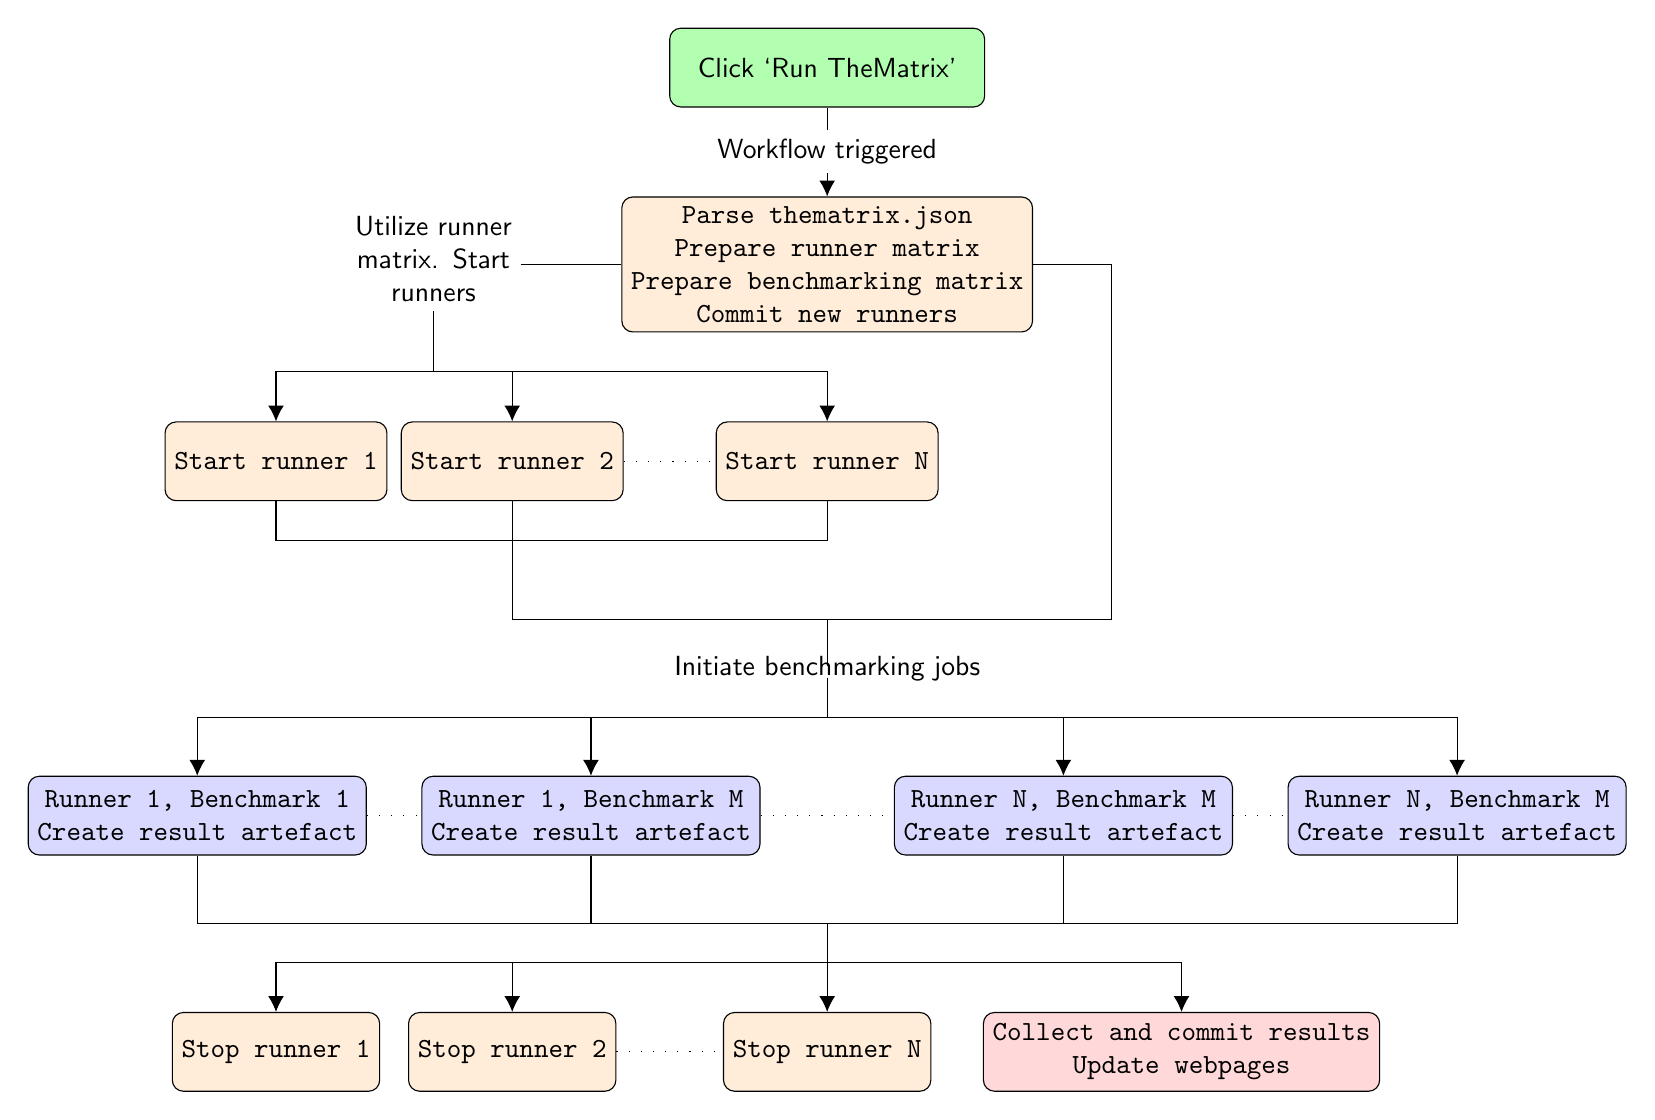
\begin{tikzpicture}[node distance=1.5cm,
    every node/.style={fill=white, font=\sffamily}, align=center]
  \node (workflowStarts)      [workflowStarts] {Click `Run TheMatrix'};
  \node (preprocessBlock)      [gitRunner, below of=workflowStarts, yshift=-1cm]
   {Parse \texttt{thematrix.json} \\ Prepare runner matrix \\ Prepare benchmarking matrix \\Commit new runners};
  \node (startRunner1)      [gitRunner, below of=preprocessBlock, xshift=-7cm, yshift=-1cm]
                                                                {Start runner 1};
  \node (startRunner2)      [gitRunner, below of=preprocessBlock, xshift=-4cm, yshift=-1cm]
                                                                {Start runner 2};
  \node (startRunnerN)      [gitRunner, below of=preprocessBlock, xshift=-0cm, yshift=-1cm]
                                                                {Start runner N};
  \node (bench11)      [shRunner, below of=startRunnerN, xshift=-8cm, yshift=-3cm]
                                                                {Runner 1, Benchmark 1 \\ Create result artefact};
  \node (bench1M)      [shRunner, below of=startRunnerN, xshift=-3cm, yshift=-3cm]
                                                                {Runner 1, Benchmark M \\ Create result artefact};
  \node (benchN1)      [shRunner, below of=startRunnerN, xshift=3cm, yshift=-3cm]
                                                                {Runner N, Benchmark M \\ Create result artefact};
  \node (benchNM)      [shRunner, below of=startRunnerN, xshift=8cm, yshift=-3cm]
                                                                {Runner N, Benchmark M \\ Create result artefact};
  \node (stopRunner1)      [gitRunner, below of=startRunner1, xshift=0cm, yshift=-6cm]
                                                                {Stop runner 1};
  \node (stopRunner2)      [gitRunner, below of=startRunner2, xshift=0cm, yshift=-6cm]
                                                                {Stop runner 2};
  \node (stopRunnerN)      [gitRunner, below of=startRunnerN, xshift=0cm, yshift=-6cm]
                                                                {Stop runner N};
  \node (publish)      [MatMul, right of=stopRunnerN, xshift=3cm, yshift=0cm]
                                                                {Collect and commit results \\ Update webpages};

  \coordinate[left=5cm of preprocessBlock.south] (auxNode1);
  \coordinate[below=0.5cm of auxNode1.south] (auxNode2);
  \coordinate[below=0.5cm of startRunner2.south] (auxNode3);
  \coordinate[right=1cm of preprocessBlock.east] (auxNode4);
  \coordinate[below=1.5cm of startRunnerN.south] (auxNode5);
  \coordinate[below=0.5cm of auxNode5.south] (auxNode6);
  \coordinate[below=0.25cm of auxNode6.south] (auxNode6a);
  \coordinate[below=0.5cm of auxNode6a.south] (auxNode6b);
  \coordinate[below=7.5cm of preprocessBlock.south] (auxNode7);
  \coordinate[below=8cm of preprocessBlock.south] (auxNode8);

  % Specification of lines between nodes
  \draw[->]      (workflowStarts) -- node[text width=4cm]
                                   {Workflow triggered} (preprocessBlock);
  \draw[-]      (preprocessBlock) -| node[text width=2cm, text height=0.1cm]
                                   {Utilize runner matrix. Start runners} (auxNode1);
  \draw[-]      (auxNode1) -| (auxNode2);
  \draw[->]      (auxNode2) -| (startRunner1);
  \draw[->]      (auxNode2) -| (startRunner2);
  \draw[->]      (auxNode2) -| (startRunnerN);
  \draw[loosely dotted]             (startRunner2) -- (startRunnerN);
  \draw[-]      (startRunner1) |- (auxNode3);
  \draw[-]      (startRunner2) |- (auxNode3);
  \draw[-]      (startRunnerN) |- (auxNode3);
  \draw[-]      (preprocessBlock) -- (auxNode4);
  \draw[-]      (auxNode4) |- (auxNode5);
  \draw[-]      (auxNode3) |- (auxNode5);
  \draw[-]      (auxNode5) |- (auxNode6);
  \draw[-]      (auxNode6) |- node[text width=4cm, text height=0cm]
                                   {Initiate benchmarking jobs} (auxNode6a);
  \draw[-]      (auxNode6a) |- (auxNode6b);
  \draw[->]      (auxNode6b) -| (bench11);
  \draw[->]      (auxNode6b) -| (bench1M);
  \draw[->]      (auxNode6b) -| (benchN1);
  \draw[->]      (auxNode6b) -| (benchNM);
  \draw[loosely dotted]             (bench11) -- (bench1M);
  \draw[loosely dotted]             (bench1M) -- (benchN1);
  \draw[loosely dotted]             (benchN1) -- (benchNM);
  \draw[-]      (bench11) |- (auxNode7);
  \draw[-]      (bench1M) |- (auxNode7);
  \draw[-]      (benchN1) |- (auxNode7);
  \draw[-]      (benchNM) |- (auxNode7);
  \draw[loosely dotted]             (stopRunner2) -- (stopRunnerN);
  \draw[-]      (auxNode7) |- (auxNode8);
  \draw[->]      (auxNode8) -| (stopRunner1);
  \draw[->]      (auxNode8) -| (stopRunner2);
  \draw[->]      (auxNode8) -| (stopRunnerN);
  \draw[->]      (auxNode8) -| (publish);
     {The activity comes to the foreground}(onResumeBlock.east);
  \end{tikzpicture}
\end{document}
